\begin{table}[H]
	\centering
	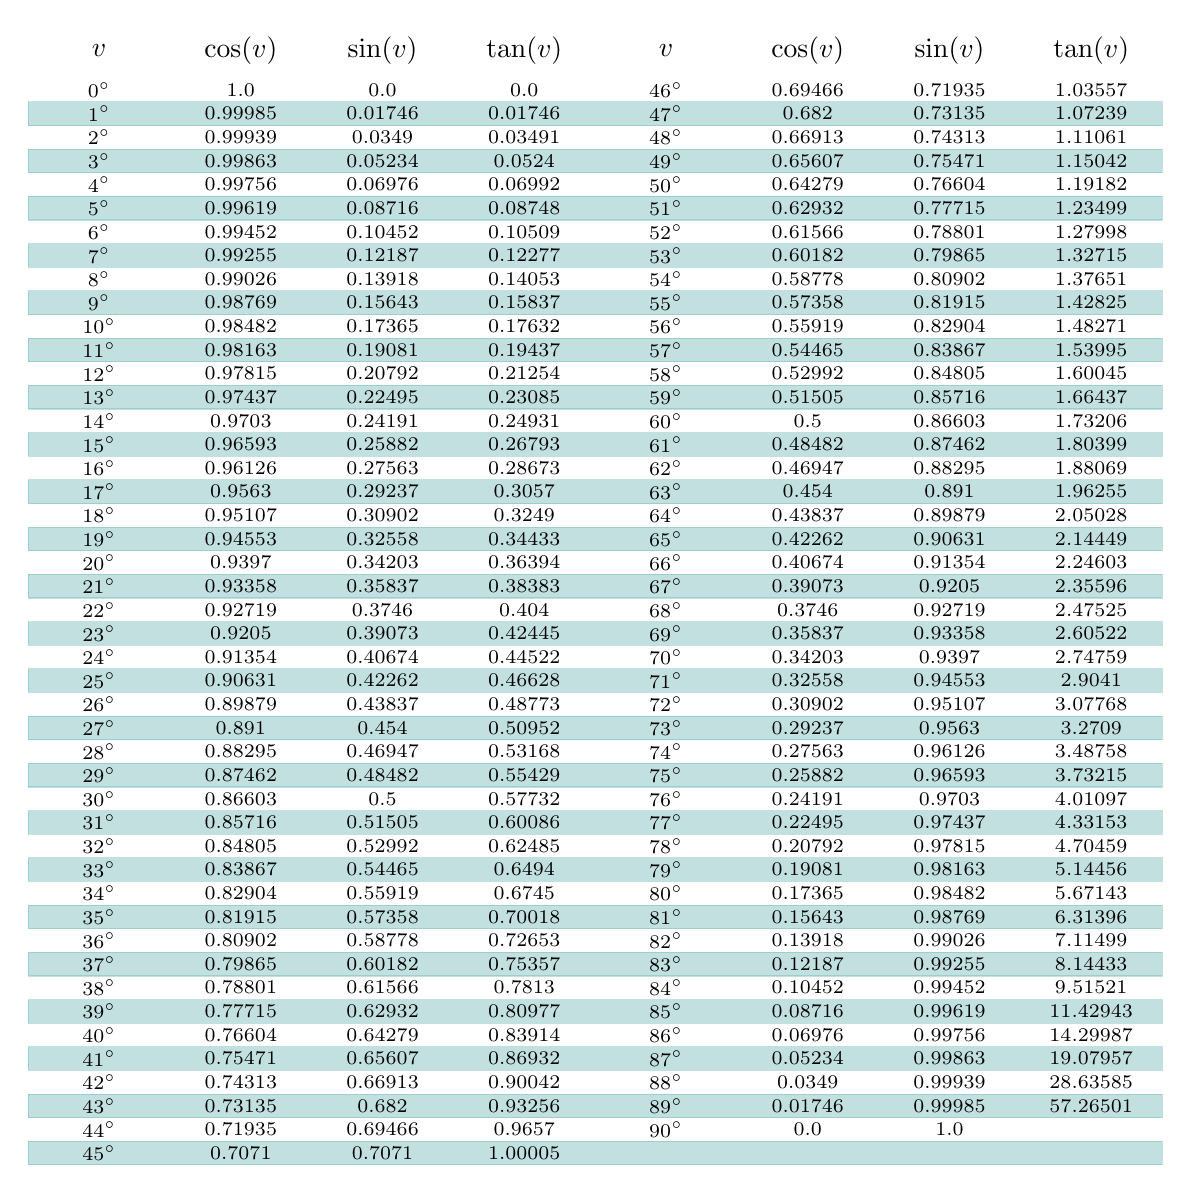
\begin{tikzpicture}
	\node at (0,0) {$v$};
	\node at (2*0.9,0) {$\cos(v)$};
	\node at (4*0.9,0) {$\sin(v)$};
	\node at (6*0.9,0) {$\tan(v)$};
	\node at (8*0.9,0) {$v$};
	\node at (10*0.9,0) {$\cos(v)$};
	\node at (12*0.9,0) {$\sin(v)$};
	\node at (14*0.9,0) {$\tan(v)$};
	\scriptsize
	%Colors
	\foreach \i in {0,...,22}{
		\filldraw[color = teal!60, opacity = 0.4] (-0.9,-0.5-0.3+0.15-\i*0.3*2) rectangle
		 (14*0.9 + 0.9,-0.5-0.3-0.15-\i*0.3*2);
	}
	\foreach \i in {0,...,45}{
		%Macros for evaluating
		\pgfmathsetmacro{\cval}{cos(\i)}
		\pgfmathsetmacro{\sval}{sin(\i)}
		\pgfmathsetmacro{\tval}{tan(\i)}
		%First columns of values
		\node at (0,-0.5-\i*0.3) {$\i^{\circ}$};
		\node at (2*0.9,-0.5-\i*0.3) { \cval };
		\node at (4*0.9,-0.5-\i*0.3) { \sval };
		\node at (6*0.9,-0.5-\i*0.3) { \tval };
	}
	\foreach \i in {46,...,89}{
		%Macros
		\pgfmathsetmacro{\cval}{cos(\i)}
		\pgfmathsetmacro{\sval}{sin(\i)}
		\pgfmathsetmacro{\tval}{tan(\i)}
		%Second column
		\node at (8*0.9,-0.5-\i*0.3 + 46*0.3) {$\i^{\circ}$};
		\node at (10*0.9,-0.5-\i*0.3 + 46*0.3) { \cval };
		\node at (12*0.9,-0.5-\i*0.3 + 46*0.3) { \sval };
		\node at (14*0.9,-0.5-\i*0.3 + 46*0.3) { \tval };
	}
		\pgfmathsetmacro{\cval}{cos(90)}
		\pgfmathsetmacro{\sval}{sin(90)}
		\node at (8*0.9,-0.5-90*0.3 + 46*0.3) {$90^{\circ}$};
		\node at (10*0.9,-0.5-90*0.3 + 46*0.3) { \cval };
		\node at (12*0.9,-0.5-90*0.3 + 46*0.3) { \sval };
	\end{tikzpicture}
	\caption{Tabel over udvalgte værdier for $\cos$, $\sin$ og $\tan$.}
	\label{tab:cossintan}
\end{table}

\newpage
\begin{figure}[H]
	\centering
	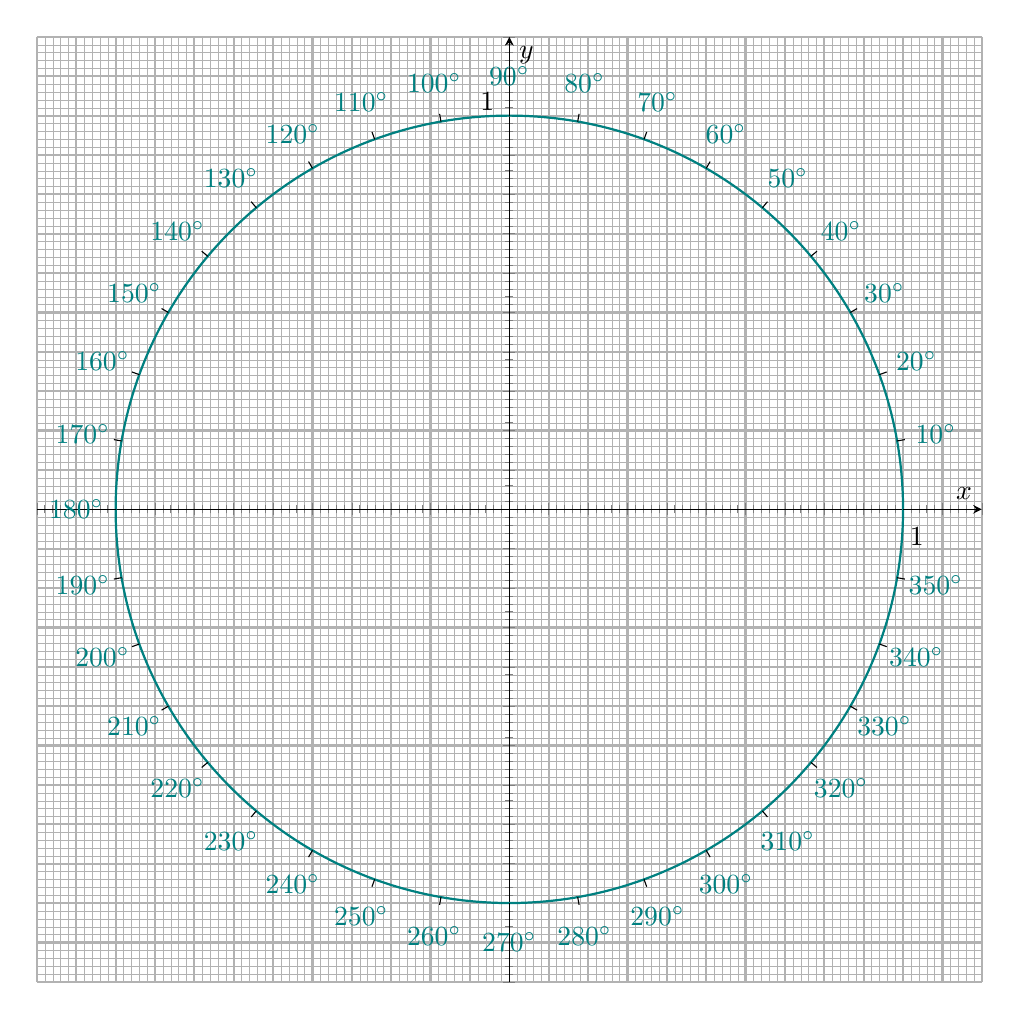
\begin{tikzpicture}
		\begin{axis}[
			axis lines = center, 
			xmin = -1.2, xmax = 1.2, 
			ymin = -1.2, ymax = 1.2, 
			x = 5cm, y = 5cm,
			major grid style={line width=0.8pt, draw=gray!60},
			minor grid style={line width=0.1pt, draw=gray!60},
			ytick distance = 0.1,
			xtick distance = 0.1,
			minor tick num = 4,
			grid = both,
			xticklabels = {},
			yticklabels = {},
			xlabel = $x$, ylabel = $y$
		]
			%Shifted tick labels since unit circle would otherwise be in the way:
			\node[xshift = 5pt, yshift = -10pt] at (axis cs:1,0) {1};
			\node[xshift = -8pt, yshift = 5pt] at (axis cs:0,1) {1};
			\draw[color = teal, thick] (axis cs:0,0) circle (5cm);
			%Ticks on circle 
			\pgfplotsinvokeforeach{0,1,...,35}
			{
				\draw (axis cs: {cos(#1*10)},{sin(#1*10)})-- (axis cs: {1.02*cos(#1*10)},{1.02*sin(#1*10)});
			}
			\pgfplotsinvokeforeach{10,20,...,350}
			{
				\node[color = teal] at (axis cs: {1.10*cos(#1)},{1.10*sin(#1)}) {$#1^\circ$};
			}
		\end{axis}
	\end{tikzpicture}
	\caption{Enhedscirkel til aflæsning af $\cos$ og $\sin$.}
	\label{fig:enhed}
\end{figure}



\subsection*{Opgave 1}

To trekanter $\triangle ABC$ og $\triangle PQR$ er givet ved
\begin{center}
\begin{tikzpicture}
	%Trekant1
	\coordinate (1) at (0,0);
	\coordinate (2) at (3,0);
	\coordinate (3) at (3.5,1.94);
	\draw[color = olive, thick] (1) -- (2)
	node[midway, anchor = north] {$6$};
	\draw[color = olive, thick] (1) -- (3)
	node[midway, anchor = south east] {$8$};
	\draw[color = olive, thick] (2) -- (3)
	node[midway, anchor = north west] {$a$};
	\node[color = olive, anchor = north east] at (1) {$A$};
	\node[color = olive, anchor = north west] at (2) {$B$};
	\node[color = olive, anchor = south] at (3) {$C$};
	\draw[color = olive, thick] (0+0.5,0) arc (0:28.96:0.5);
	\draw[color = olive, thick] (3-0.4,0) arc (180:180-104.48:0.4);
	\draw[color = olive, thick] (3-0.5,0) arc (180:180-104.48:0.5);
	 
	%Trekant2
	\coordinate (4) at (0+5,0);
	\coordinate (5) at (3*2+5,0);
	\coordinate (6) at (3.5*2 + 5,1.94*2);
	\draw[color = olive, thick] (4) -- (5)
	node[midway, anchor = north] {$r$};
	\draw[color = olive, thick] (4) -- (6)
	node[midway, anchor = south east] {$24$};
	\draw[color = olive, thick] (5) -- (6)
	node[midway, anchor = north west] {$12$};
	\node[color = olive, anchor = north east] at (4) {$P$};
	\node[color = olive, anchor = north west] at (5) {$Q$};
	\node[color = olive, anchor = south] at (6) {$R$};
	\draw[color = olive, thick] (0+0.5+5,0) arc (0:28.96:0.5);
	\draw[color = olive, thick] (3*2-0.4+5,0) arc (180:180-104.48:0.4);
	\draw[color = olive, thick] (3*2-0.5+5,0) arc (180:180-104.48:0.5);
	\end{tikzpicture}
\end{center}
\begin{enumerate}[label=\roman*)]
	\item Bestem skalafaktoren $k$ samt længden af siderne $a$ og $r$.
\end{enumerate}

\subsection*{Opgave 2}

En retvinklet trekant $\triangle ABC$ opfylder, at $a = 8$, $c = 10$ og $\angle C = 90$.
\begin{enumerate}[label=\roman*)]
	\item Bestem sidelængden $b$.
\end{enumerate}

\subsection*{Opgave 3 (med hjælpemidler)}
Bestem de ukendte sider og vinkler i følgende trekanter:
\begin{center}
\begin{tikzpicture}
\node at (0,0) (1) {$A$};
\node at (5,0) (2) {$C$};
\node at (5,3)(3)	{$B$};
\node at (1.2,0.3) (4)   {\scriptsize $45^\circ$};
\node at (2.5,-0.5)  {$8$};


\draw (1) -- (2);
\draw (2) -- (3);
\draw (3) -- (1);
\end{tikzpicture}

\begin{tikzpicture}
\node at (0,0) (1) {$A$};
\node at (4,0) (2) {$C$};
\node at (4,4) (3)	{$B$};
\node at (1.2,0.3)  {};% {\scriptsize $30^\circ$};
\node at (2,-0.5)  {$9$};
\node at (1.8,2.2)   {$12$};

\draw (1) -- (2);
\draw (2) -- (3);
\draw (3) -- (1);
\end{tikzpicture}


\begin{tikzpicture}
\node at (0,0) (1) {$A$};
\node at (3,0) (2) {$C$};
\node at (3,6) (3)	{$B$};
\node at (1.5,-0.3)  {$10$};
\node at (3.3,3)  {$20$};


\draw (1) -- (2);
\draw (2) -- (3);
\draw (3) -- (1);
\end{tikzpicture}
\end{center}



\subsection*{Opgave 4}
Brug Tabel \ref{tab:cossintan} til at bestemme vinklen i følgende trekanter. 


\begin{center}
	\begin{minipage}{0.45\textwidth}
		\centering
		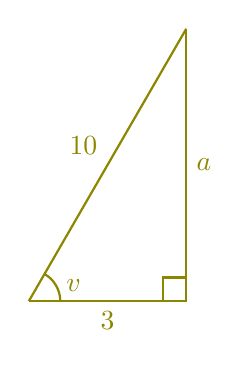
\begin{tikzpicture}
		\draw[color = olive, thick] (0,0) -- (2,0) node[midway, anchor = north] {$3$};
		\draw[color = olive, thick] (0,0) -- (2,3.46) node[midway, anchor = south east] {$10$};
		\draw[color = olive, thick] (2,0) -- (2,3.46) node[midway, anchor = west] {$a$};
		\draw[color = olive, thick] (0.4,0) arc (0:60:0.4) node[midway, anchor = west] {$v$};
		\draw[color = olive, thick] (2,0) rectangle (2-0.3,0.3);
		\end{tikzpicture}
	\end{minipage}
	\begin{minipage}{0.45\textwidth}
		\centering
		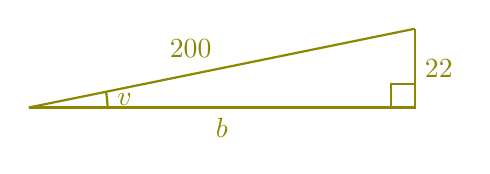
\begin{tikzpicture}
		\draw[color = olive, thick] (0,0) -- (4.9,0) node[midway, anchor = north] {$b$};
		\draw[color = olive, thick] (0,0) -- (4.9,1) node[midway, anchor = south east] {$200$};
		\draw[color = olive, thick] (4.9,0) -- (4.9,1) node[midway, anchor = west] {$22$};
		\draw[color = olive, thick] (1,0) arc (0:11.52:1) node[midway, anchor = west] {$v$};
		\draw[color = olive, thick] (4.9,0) rectangle (4.9-0.3,0.3);
		\end{tikzpicture}
	\end{minipage}
\end{center}

\subsection*{Opgave 5 (med hjælpemidler)}
En trekant $\triangle ABC$ opfylder, at $\angle A = 25^\circ$, $c = 10$ og $b = 17$
\begin{enumerate}[label=\roman*)]
	\item Bestem arealet af $\triangle ABC$.
	\item Hvis $c$ er trekantens grundlinje, hvor høj er trekanten så?
\end{enumerate}

\subsection*{Opgave 6 (med hjælpemidler)}

En trekant $\triangle ABC$ opfylder, at $\angle A = 70^\circ$, $\angle B = 22^\circ$ og $a = 5$.
\begin{enumerate}[label= \roman*)]
	\item Bestem de resterende sidelængder og vinkler i trekanten.
\end{enumerate}

\subsection*{Opgave 7}
En trekant $\triangle ABC$ opfylder, at $\angle A = 30^\circ$ og $\angle C = 90^\circ$. 
\begin{enumerate}[label=\roman*)]
	\item Hvor mange gange længere er sidelængden $c$ end sidelængden $a$?
\end{enumerate}

\subsection*{Opgave 8 (med hjælpemidler)}
En trekant $\triangle ABC$ opfylder, at $a = 10$, $b = 7$ og $c = 13$. 
\begin{enumerate}[label=\roman*)]
	\item Bestem vinklerne i trekanten $\triangle ABC$. 
\end{enumerate}

\subsection*{Opgave 9}
Vi skal argumentere for, at $\cos(60) = 0.5$. 
\begin{enumerate}[label=\roman*)]
	\item Tegn en enhedscirken med en linje ud til randen af cirklen,
	 der danner en vinkel med $x$-aksen på $60^\circ$.
	\item Tegn en retvinklet trekant, hvor dette er hypotenusen og
	 den hosliggende katete har længden $\cos(60)$.
	\item Hvad er vinklerne i denne trekant?
	\item Kan du tegne en trekant ved siden af denne trekant, der sammen med denne trekant
	 viser at $\cos(60) = 0.5$?
\end{enumerate}
Vi skal nu vise, at $\sin(60) = \frac{\sqrt{3}}{2}$
\begin{enumerate}[label=\roman*)]
	\setcounter{enumi}{4}
\item Indsæt $\cos(60)$ og $\sin(60)$ i idiotformlen og isolér $\sin(60)$. 
\item Kan du argumentere for, at $\sin(30) = 0.5$ og $\cos(30) = \frac{\sqrt{3}}{2}$?
\end{enumerate}
